\begin{figure}
  \centering
  \begin{tabular}{cc}
    \begin{minipage}{0.5\hsize}
      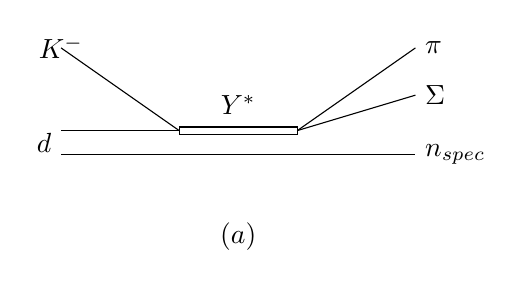
\begin{tikzpicture}[scale=1.5]
        \draw (-1.5,    0.7) node {$K^-$}--(-0.5,    0);
        \draw (-1.5,    0)--(-0.5,    0);
        \draw (-0.5, 0.03) rectangle (0.5, -0.03);
        \draw (0.0, 0.05) node [above]{$Y^*$};
        \draw (0.5, 0)--(1.5, 0.3) node [right] {$\Sigma$};
        \draw (0.5, 0)--(1.5, 0.7) node [right] {$\pi$};
        
        \draw (-1.5, -0.2)--(1.5, -0.2) node [right] {$n_{spec}$};
        \node (d) at (-1.5, -0.1) [left] {$d$};

        \draw (0, -0.7) node [below] {$(a)$};
      \end{tikzpicture}
    \end{minipage}

    \begin{minipage}{0.5\hsize}
      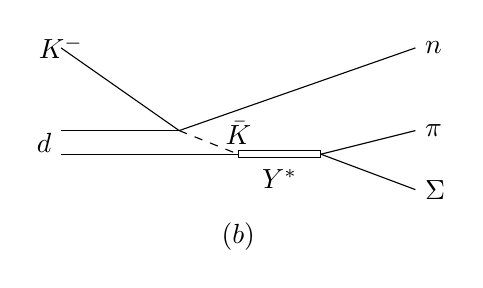
\begin{tikzpicture}[scale=1.5]
        \draw (-1.5,    0.7) node {$K^-$}--(-0.5,    0);
        \draw (-1.5,    0)--(-0.5,    0);
        \draw (-1.5, -0.2)--(0.0, -0.2);
        \node (d) at (-1.5, -0.1) [left] {$d$};
        
        \draw (-0.5, 0) -- (0.0, -0.2) [dashed];
        \node (barK) at (0.0, -0.2) [above] {$\bar{K}$};

        \draw ( -0.0, -0.23) rectangle (0.7, -0.17);
        \draw ( 0.35, -0.25) node [below] {$Y^*$};
        
        \draw ( 1.5,  -0.5) node [right] {$\Sigma$} -- (0.7, -0.2);
        \draw ( 1.5,  -0.0) node [right] {$\pi$}    -- (0.7, -0.2);
        \draw ( 1.5,  0.7) node [right] {$n$}      -- (-0.5,    0);
        \draw (0, -0.7) node [below] {$(b)$};
      \end{tikzpicture}
    \end{minipage}
  \end{tabular}
  \caption{
    This figure is a diagram of the $K^-d\rightarrow n \Sigma \pi$ reaction.
    The left figure (a) represents a one-nucleon reaction, and the right figure (b) represents a two-step reaction.    
  }
  \label{fig:kd_diag}
\end{figure}

Given the aforementioned circumstances, it is strongly desired to measure direct $\bar{K}N$ scattering data in the mass region of $\Lambda(1405)$.
However, if the scattered $\bar{K}$ meson and nucleon are detected as free particles after $\bar{K}N$ scattering,
scattering amplitudes below the $\bar{K}N$ mass threshold cannot be obtained.
As stated in Section \ref{sec:KN_interaction}, while the $K^-p$ reaction provides scattering data above the $\bar{K}N$ mass threshold,
it cannot provide scattering amplitudes below the threshold due to energy conservation.
Thus, the $K^-d \rightarrow n Y^*$ reaction with a deuterium target can be used,
in which $Y^*$ can be produced below the $\bar{K}N$ mass threshold by transferring the energy of the $K^-$ beam to the neutron.

Experiments using this reaction were conducted at CERN by irradiating a liquid deuterium target with a $K^-$ beam having a momentum of 686-844 MeV$/c$ \cite{Braun}.
Although only the spectrum of the $\pi^+\Sigma^-$ mode was reported in this experiment,
the spectrum showed a peak around 1420 MeV, which is higher than the conventional peak position of $\Lambda(1405)$.
Since this reaction is $\bar{K}$-induced, it is considered to strongly reflect the $\bar{K}N$ pole,
which is consistent with the chiral unitary model.
In fact, D. Jido et al. used the chiral unitary model to calculate the $K^- d \rightarrow n \Sigma \pi$ reaction
and successfully reproduced the experimental spectrum \cite{Jido2}.
However, their calculation also required the $P$-wave $\Sigma(1385)$ contribution at $I=1$.
The $\pi \Sigma$ spectrum is reported only for $\pi^+\Sigma^-$ in this experiment,
but a $\pi^- \Lambda$ spectrum from the $K^- d \rightarrow p \Lambda \pi^-$ reaction was also reported.
Since this spectrum corresponds to $I = 1$, it does not include a $\Lambda(1405)$ contribution but does contain a $\Sigma(1385)$ contribution.
J. Yamagata et al. reproduced the $\pi^-\Lambda$ spectrum of this experiment using the same reaction calculation framework \cite{Yamagata}.
Thus, this experiment provides strong support for the validity of the chiral unitary model.

Two types of reactions are possible for this process: a one-nucleon reaction (a) and a two-step reaction (b), as shown in Figure \ref{fig:kd_diag}.
These two reactions are kinematically distinguishable, but not in this experiment, where all Y⁎ production angles were measured.
Nevertheless, neutrons originating from Fermi motion, which do not contribute directly to the reaction, are emitted in all directions.
Therefore, the one-nucleon reaction is considered to play a more significant contribution in this experiment.

Summarized, only the $\pi^-\Sigma^+$ spectrum was reported in this experiment, and the reaction mechanism remained unknown.
The J-PARC E31 experiment was planned to address this issue.

